\section{Неравенства решения}
1. $\cfrac{(x^2-4x+3)(x-3)(x^2+2x+3)}{(x^2+x-20)(x+2)^2}\geqslant0 \Leftrightarrow \cfrac{(x-1)(x-3)^2((x+1)^2+2)}{(x-4)(x+5)(x+2)^2}\geqslant0.$ Применив метод интервалов, найдём ответ: $x\in(-5;-2)\cup(-2;1]\cup\{3\}\cup(4;+\infty).$
{{PIC:ner9-1.png}}\\
2. $\cfrac{(x^2-8x+15)(x-5)(x^2-2x+3)}{(x^2-3x-18)(x+1)^2}\geqslant0\Leftrightarrow\cfrac{(x-3)(x-5)^2((x-1)^2+2)}{(x-6)(x+3)(x+1)^2}\geqslant0.$ Применив метод интервалов, найдём ответ: $x\in(-3;-1)\cup(-1;3]\cup\{5\}\cup(6;+\infty).$
{{PIC:ner9-2.png}}\\
3. $\cfrac{x(x^2+2)(2-x)(x^3-64)}{(x^2-16)(x+2)^2}\leqslant 0 \Leftrightarrow \cfrac{x(2-x)(x-4)(x^2+4x+16)}{(x-4)(x+4)(x+2)^2}\leqslant 0.$ Применив метод интервалов, найдём ответ: $x\in(-4;-2)\cup(-2;0]\cup[2;4)\cup(4;+\infty).$
{{PIC:ner9-3.png}}\\
4. $\cfrac{x(x^2+3)(3-x)(x^3-8)}{(x^2-4)(x+3)^2}\leqslant 0 \Leftrightarrow \cfrac{x(3-x)(x-2)(x^2+2x+4)}{(x-2)(x+2)(x+3)^2}\leqslant 0.$ Применив метод интервалов, найдём ответ: $x\in(-2;0]\cup[3;+\infty).$
{{PIC:ner9-4.png}}\\
5. $\cfrac{x^2+3}{x+1}\leqslant2 \Leftrightarrow \cfrac{x^2+3-2x-2}{x+1} \leqslant0\Leftrightarrow \cfrac{(x-1)^2}{x+1} \leqslant0.$ Применив метод интервалов, найдём ответ: $x\in(-\infty;-1)\cup\{1\}.$\\
6. $\cfrac{x^2}{x-1}\leqslant4 \Leftrightarrow \cfrac{x^2-4x+4}{x-1}\leqslant0 \Leftrightarrow \cfrac{(x-2)^2}{x-1}\leqslant0.$ Применив метод интервалов, найдём ответ: $x\in(-\infty;1)\cup\{2\}.$\\
7. $|2x+4|<2|x|+x \Leftrightarrow \left[\begin{array}{l}\begin{cases}-2x-4<-2x+x,\\ x\leqslant-2.\end{cases}\\ \begin{cases}2x+4<-2x+x,\\ -2<x<0.\end{cases}\\ \begin{cases}2x+4<2x+x,\\ x\geqslant0.\end{cases} \end{array}\right.\Leftrightarrow \left[\begin{array}{l}\begin{cases}x>-4,\\ x\leqslant-2.\end{cases}\\ \begin{cases}x<-\cfrac{4}{3},\\ -2<x<0.\end{cases}\\ \begin{cases}x>4,\\ x\geqslant0.\end{cases} \end{array}\right.\Leftrightarrow
x\in\left(-4;-\cfrac{4}{3}\right)\cup(4;+\infty).$\\
8. $|3x+6|<3|x|+x \Leftrightarrow \left[\begin{array}{l}\begin{cases}-3x-6<-3x+x,\\ x\leqslant-2.\end{cases}\\ \begin{cases}3x+6<-3x+x,\\ -2<x<0.\end{cases}\\ \begin{cases}3x+6<3x+x,\\ x\geqslant0.\end{cases} \end{array}\right.\Leftrightarrow \left[\begin{array}{l}\begin{cases}x>-6,\\ x\leqslant-2.\end{cases}\\ \begin{cases}x<-\cfrac{6}{5},\\ -2<x<0.\end{cases}\\ \begin{cases}x>6,\\ x\geqslant0.\end{cases} \end{array}\right.\Leftrightarrow
x\in\left(-6;-\cfrac{6}{5}\right)\cup(6;+\infty).$\\
9. $\cfrac{(x-2)(x-3)}{(x-1)^2}\geqslant0.$ Применив метод интервалов, найдём ответ: $x\in(-\infty;1)\cup(1;2]\cup[3;+\infty).$
{{PIC:ner9-9.png}}\\
10. $\cfrac{(x+2)(x+3)}{(x+1)^2}\geqslant0.$ Применив метод интервалов, найдём ответ: $x\in(-\infty;-3]\cup[-2;-1)\cup(-1;+\infty).$
{{PIC:ner9-10.png}}\\
11. $|x^2-16|\leqslant8-2x \Leftrightarrow \begin{cases} x^2-16\leqslant8-2x,\\ x^2-16\geqslant2x-8.\end{cases} \Leftrightarrow
\begin{cases} x^2+2x-24\leqslant0,\\ x^2-2x-8\geqslant0.\end{cases}\Leftrightarrow\begin{cases} (x-4)(x+6)\leqslant0,\\ (x-4)(x+2)\geqslant0.\end{cases}
\Leftrightarrow\begin{cases} x\in[-6;4],\\ x\in(-\infty;-2]\cup[4;+\infty).\end{cases}\Leftrightarrow x\in[-6;-2]\cup\{4\}.$\\
12. $|x^2-16|\leqslant8+2x \Leftrightarrow \begin{cases} x^2-16\leqslant8+2x,\\ x^2-16\geqslant-2x-8.\end{cases} \Leftrightarrow
\begin{cases} x^2-2x-24\leqslant0,\\ x^2+2x-8\geqslant0.\end{cases}\Leftrightarrow\begin{cases} (x+4)(x-6)\leqslant0,\\ (x+4)(x-2)\geqslant0.\end{cases}
\Leftrightarrow\begin{cases} x\in[-4;6],\\ x\in(-\infty;-4]\cup[2;+\infty).\end{cases}\Leftrightarrow x\in\{-4\}\cup[2;6].$\\
13. $\cfrac{(x+1)(x+2)}{x^2+7x+12}\leqslant1 \Leftrightarrow \cfrac{x^2+2x+x+2-x^2-7x-12}{x^2+7x+12}\leqslant0 \Leftrightarrow
\cfrac{-4\left(x+\cfrac{5}{2}\right)}{(x+4)(x+3)}\leqslant0.$ Применив метод интервалов, найдём ответ: $x\in(-4;-3)\cup\left[-\cfrac{5}{2};+\infty\right)$
{{PIC:ner9-13.png}}\\
14. $\cfrac{x^2+3x-13}{(x+3)(x-2)}>2 \Leftrightarrow \cfrac{x^2+3x-13-2x^2+4x-6x+12}{(x+3)(x-2)}>0\Leftrightarrow \cfrac{-(x^2-x+1)}{(x+3)(x-2)}>0
\Leftrightarrow x\in(-3;2).$\\
15. $1,5x-|x|+|2x-4|\geqslant4\Leftrightarrow 1,5x+|2x-4|\geqslant |x|+4\Leftrightarrow \left[\begin{array}{l} \begin{cases} 1,5x-2x+4\geqslant -x+4,\\
x\leqslant0.\end{cases}\\ \begin{cases} 1,5x-2x+4\geqslant x+4,\\ 0<x<2.\end{cases} \\ \begin{cases} 1,5x+2x-4\geqslant x+4,\\ 2\leqslant x.\end{cases}\end{array}\right.
\Leftrightarrow \left[\begin{array}{l} \begin{cases} x\geqslant 0,\\
x\leqslant0.\end{cases}\\ \begin{cases} x\leqslant 0,\\ 0<x<2.\end{cases} \\ \begin{cases} x\geqslant \cfrac{16}{5},\\ 2\leqslant x.\end{cases}\end{array}\right.
\Leftrightarrow x\in \{0\}\cup\left[\cfrac{16}{5};+\infty\right).$\\
16. $2x-5+2|x-3|<|x+1|\Leftrightarrow \left[\begin{array}{l} \begin{cases} 2x-5-2x+6< -x-1,\\
x\leqslant-1.\end{cases}\\ \begin{cases} 2x-5-2x+6< x+1,\\ -1<x<3.\end{cases} \\ \begin{cases} 2x-5+2x-6< x+1,\\ 3\leqslant x.\end{cases}\end{array}\right.
\Leftrightarrow \left[\begin{array}{l} \begin{cases} x< -2,\\
x\leqslant-1.\end{cases}\\ \begin{cases} x> 0,\\ -1<x<3.\end{cases} \\ \begin{cases} x<4,\\ 3\leqslant x.\end{cases}\end{array}\right.
\Leftrightarrow$\\$ x\in (-\infty;-2)\cup(0;4).$\\
17. $\cfrac{2x^2+3x-13}{(x+3)(x-2)}>2\Leftrightarrow\cfrac{2x^2+3x-13-2x^2+4x-6x+12}{(x+3)(x-2)}>0\Leftrightarrow \cfrac{x-1}{(x+3)(x-2)}>0.$
Применив метод интервалов, найдём ответ: $x\in(-3;1)\cup(2;+\infty).$
{{PIC:ner9-17.png}}\\
18. $|x^2-7x+7|>x-5\Leftrightarrow \left[\begin{array}{l} x^2-7x+7>x-5,\\ x^2-7x+7<-x+5.\end{array}\right.\Leftrightarrow
\left[\begin{array}{l} x^2-8x+12>0,\\ x^2-6x+2<0.\end{array}\right.\Leftrightarrow$\\$
\left[\begin{array}{l} (x-6)(x-2)>0,\\ (x-(3+\sqrt{7}))(x-(3-\sqrt{7}))<0.\end{array}\right.\Leftrightarrow
\left[\begin{array}{l} x\in(-\infty;2)\cup(6;+\infty),\\ x\in(3-\sqrt{7};3+\sqrt{7}).\end{array}\right.\Leftrightarrow
x\in (-\infty;3+\sqrt{7})\cup(6;+\infty).$\\
19. $|x^2-4x-14|<x+10\Leftrightarrow \begin{cases}x^2-4x-14<x+10,\\ x^2-4x-14>-x-10.\end{cases}\Leftrightarrow
\begin{cases}x^2-5x-24<0,\\ x^2-3x-4>0.\end{cases}\Leftrightarrow$\\$
\begin{cases}(x-8)(x+3)<0,\\ (x-4)(x+1)>0.\end{cases}\Leftrightarrow
\begin{cases}x\in(-3;8),\\ x\in(-\infty;-1)\cup(4;+\infty).\end{cases}\Leftrightarrow x\in (-3;-1)\cup(4;8).$\\
20. $\cfrac{(x-1)(x-2)}{x^2+7x+12}\leqslant1\Leftrightarrow \cfrac{x^2-2x-x+2-x^2-7x-12}{x^2+7x+12}\leqslant0
\Leftrightarrow \cfrac{-10(x+1)}{(x+3)(x+4)}\leqslant0.$ Применив метод интервалов, найдём ответ: $x\in(-4;-3)\cup[-1;+\infty).$
{{PIC:ner9-20.png}}\\
21. $\cfrac{(x-1)(x+3)}{x^2+7x+12}\leqslant1\Leftrightarrow \cfrac{x^2+3x-x-3-x^2-7x-12}{x^2+7x+12}\leqslant0
\Leftrightarrow \cfrac{-5(x+3)}{(x+3)(x+4)}\leqslant0\Leftrightarrow \begin{cases} x+4>0,\\ x\neq-3.\end{cases}
\Leftrightarrow x\in(-4;-3)\cup(-3;+\infty).$\\
22. $\cfrac{x^2-2x-8}{|x-4|}<7\Leftrightarrow\cfrac{(x-4)(x+2)}{|x-4|}<7\Leftrightarrow \left[\begin{array}{l} \begin{cases}x+2<7,\\ x>4.\end{cases}\\
\begin{cases}x+2>-7,\\ x<4.\end{cases}\end{array}\right.\Leftrightarrow  x\in (-9;4)\cup(4;5).$\\
23. $\cfrac{x^2-4x-5}{|x-5|}<7\Leftrightarrow\cfrac{(x-5)(x+1)}{|x-5|}<7\Leftrightarrow \left[\begin{array}{l} \begin{cases}x+1<7,\\ x>5.\end{cases}\\
\begin{cases}x+1>-7,\\ x<5.\end{cases}\end{array}\right.\Leftrightarrow  x\in (-8;5)\cup(5;6).$\\
24. $\cfrac{x^2+9x+20}{(2x-x^2-1)(3x^2+x+2)}\leqslant0\Leftrightarrow \cfrac{(x+4)(x+5)}{-(x-1)^2\left(\left(x+\cfrac{1}{2}\right)^2+2x^2+\cfrac{3}{4}\right)}\leqslant0.$ Применив метод интервалов, найдём ответ: $x\in
(-\infty;-5]\cup[-4;1)\cup(1;+\infty).$
{{PIC:ner9-24.png}}\newpage\noindent
25. $\cfrac{(2x^2+x+1)(6x-x^2-9)}{x^2+8x+15}\geqslant0\Leftrightarrow \cfrac{-\left(\left(x+\cfrac{1}{2}\right)+x^2+\cfrac{3}{4}\right)(x-3)^2}{(x+3)(x+5)}\geqslant0.$ Применив метод интервалов, найдём ответ: $x\in
(-5;-3)\cup\{3\}.$
{{PIC:ner9-25.png}}\\
26. $\cfrac{(x^2-2x-8)(x^2-4x)}{x^2+7x+10}>0\Leftrightarrow\cfrac{x(x-4)^2(x+2)}{(x+2)(x+5)}>0.$ Применив метод интервалов, найдём ответ: $x\in
(-\infty;-5)\cup(0;4)\cup(4;+\infty).$
{{PIC:ner9-26.png}}\\
27. $\cfrac{(x^2-6x+8)(x^2-4)}{x^3+8}\geqslant0\Leftrightarrow \cfrac{(x-4)(x-2)^2(x+2)}{(x+2)(x^2-2x+4)}\geqslant0.$ Применив метод интервалов, найдём ответ: $x\in\{2\}\cup[4;+\infty).$
{{PIC:ner9-27.png}}\\
28. $x^2-2x-8<7|x-4|\Leftrightarrow \left[\begin{array}{l} 7x-28>x^2-2x-8,\\ 7x-28<-x^2+2x+8.\end{array}\right.\Leftrightarrow
\left[\begin{array}{l} x^2-9x-20<0,\\ x^2+5x-36<0.\end{array}\right.\Leftrightarrow$\\$
\left[\begin{array}{l} (x-5)(x-4)<0,\\ (x-4)(x+9)<0.\end{array}\right.\Leftrightarrow
\left[\begin{array}{l} x\in(4;5),\\ x\in(-9;4).\end{array}\right.\Leftrightarrow x\in (-9;4)\cup(4;5).$\\
29. $|x^2-3x|+2x-6\leqslant0\Leftrightarrow|x^2-3x|\leqslant6-2x\Leftrightarrow \begin{cases} x^2-3x\leqslant6-2x,\\ x^2-3x\geqslant2x-6.\end{cases}
\Leftrightarrow \begin{cases} x^2-x-6\leqslant0,\\ x^2-5x+6\geqslant0.\end{cases}
\Leftrightarrow \begin{cases} (x-3)(x+2)\leqslant0,\\ (x-3)(x-2)\geqslant0.\end{cases}
\Leftrightarrow \begin{cases} x\in[-2;3],\\ x\in(-\infty;2]\cup[3;+\infty).\end{cases}\Leftrightarrow x \in [-2;2]\cup\{3\}.$\newpage\noindent
30. $\cfrac{(x^2-4x+4)(9-x^2)}{x^2+8x+16}\leqslant0\Leftrightarrow\cfrac{-(x-2)^2(x-3)(x+3)}{(x+4)^2}\leqslant0.$ Применив метод интервалов, найдём ответ: $x\in
(-\infty;-4)\cup(-4;-3]\cup\{2\}\cup[3;+\infty).$
{{PIC:ner9-30.png}}\\
31. $\cfrac{(x^2+14x+49)(16-x^2)}{x^2-6x+9}\geqslant0\Leftrightarrow\cfrac{-(x+7)^2(x-4)(x+4)}{(x-3)^2}\geqslant0.$ Применив метод интервалов, найдём ответ: $x\in
\{-7\}\cup[-4;3)\cup(3;4].$
{{PIC:ner9-31.png}}\\
32. $\cfrac{(1-x^2)(x-1)^2(x+1)^3}{x^6+x^4+x^2}\leqslant0\Leftrightarrow\cfrac{-(x-1)^3(x+1)^4}{x^2(x^4+x^2+1)}\leqslant0.$ Применив метод интервалов, найдём ответ: $x\in\{-1\}\cup[1;+\infty).$
{{PIC:ner9-32.png}}\\
33. $\cfrac{(-1+x^2)(1-x)^2(x+1)^3}{x^8-x^6+x^4}\leqslant0\Leftrightarrow\cfrac{(x-1)^3(x+1)^4}{x^4(x^4-x^2+1)}\leqslant0.$ Применив метод интервалов, найдём ответ: $x\in(-\infty;0)\cup(0;1].$
{{PIC:ner9-33.png}}\\
34. $\left|\cfrac{x-1}{x+2}\right|>1\Leftrightarrow \left[\begin{array}{l} \cfrac{x-1}{x+2}>1,\\ \cfrac{x-1}{x+2}<-1.\end{array}\right.\Leftrightarrow
\left[\begin{array}{l} \cfrac{x-1-x-2}{x+2}>0,\\ \cfrac{x-1+x+2}{x+2}<0.\end{array}\right.\Leftrightarrow
\left[\begin{array}{l} \cfrac{-3}{x+2}>0,\\ \cfrac{2x+1}{x+2}<0.\end{array}\right.\Leftrightarrow
\left[\begin{array}{l} x<-2,\\ -2<x<-\cfrac{1}{2}.\end{array}\right.\Leftrightarrow$\\$
 x\in (-\infty;-2)\cup\left(-2;-\cfrac{1}{2}\right).$\\
35. $\left|\cfrac{x+2}{x-1}\right|<1\Leftrightarrow \begin{cases} \cfrac{x+2}{x-1}<1,\\ \cfrac{x+2}{x-1}>-1.\end{cases}\Leftrightarrow
\begin{cases} \cfrac{x+2-x+1}{x-1}<0,\\ \cfrac{x+2+x-1}{x-1}>0.\end{cases}\Leftrightarrow
\begin{cases} \cfrac{3}{x-1}<0,\\ \cfrac{2x+1}{x-1}>0.\end{cases}\Leftrightarrow$\\$
\begin{cases} x<1,\\ x\in\left(-\infty;-\cfrac{1}{2}\right)\cup(1;+\infty).\end{cases}\Leftrightarrow
 x\in \left(-\infty;-\cfrac{1}{2}\right).$\\
36. $\cfrac{(x+1)\sqrt{-x^2-10x+11}}{x^2+x-12}\geqslant0\Leftrightarrow \cfrac{(x+1)\sqrt{-(x+11)(x-1)}}{(x+4)(x-3)}\geqslant0.$ Применив метод интервалов, найдём ответ: $x\in\{-11;1\}\cup(-4;-1].$
{{PIC:ner9-36.png}}\\
37. $\cfrac{(x+2)\sqrt{-x^2-10x+11}}{x^2+x-12}\geqslant0\Leftrightarrow\cfrac{(x+2)\sqrt{-(x+11)(x-1)}}{(x+4)(x-3)}\geqslant0.$ Применив метод интервалов, найдём ответ: $x\in\{-11;1\}\cup(-4;-2].$
{{PIC:ner9-37.png}}\\
38. $\cfrac{4}{\sqrt{x-5}+3}>\cfrac{3}{\sqrt{x-5}+4}.$ У левой дроби больше числитель и меньше знаменатель, значит неравенство верно на всей ОДЗ, то есть $x\in[5;+\infty).$\\
39. $\cfrac{3}{\sqrt{x-4}+2}>\cfrac{2}{\sqrt{x-4}+3}.$ У левой дроби больше числитель и меньше знаменатель, значит неравенство верно на всей ОДЗ, то есть $x\in[4;+\infty).$\\
40. $\cfrac{x^2-4x+3}{2x-3}\leqslant\cfrac{x^2-4x+3}{x-2}\Leftrightarrow (x^2-4x+3)\left(\cfrac{1}{2x-3}-\cfrac{1}{x-2}\right)\leqslant0
\Leftrightarrow (x^2-4x+3)\cdot\cfrac{x-2-2x+3}{(2x-3)(x-2)}\leqslant0\Leftrightarrow\cfrac{-(x-3)(x-1)^2}{(2x-3)(x-2)}\leqslant0.$ Применив метод интервалов, найдём ответ: $x\in\{1\}\cup\left(\cfrac{3}{2};2\right)\cup[3;+\infty).$
{{PIC:ner9-40.png}}\newpage\noindent
41. $\cfrac{x^2-3x+2}{2x+3}\leqslant\cfrac{x^2-3x+2}{x+5}\Leftrightarrow (x^2-3x+2)\left(\cfrac{1}{2x+3}-\cfrac{1}{x+5}\right)\leqslant0
\Leftrightarrow (x^2-3x+2)\cdot\cfrac{x+5-2x-3}{(2x+3)(x+5)}\leqslant0\Leftrightarrow\cfrac{-(x-1)(x-2)^2}{(2x+3)(x+5)}\leqslant0.$ Применив метод интервалов, найдём ответ: $x\in\left(-5;-\cfrac{3}{2}\right)\cup[1;+\infty).$
{{PIC:ner9-41.png}}\\
42. $\cfrac{(x+3)^2(x^2+4x-5)}{x^2-8x+16}\geqslant0\Leftrightarrow\cfrac{(x+3)^2(x+5)(x-1)}{(x-4)^2}\geqslant0.$ Применив метод интервалов, найдём ответ: $x\in(-\infty;-5]\cup\{-3\}\cup[1;4)\cup(4;+\infty).$
{{PIC:ner9-42.png}}\\
43. $\cfrac{(x-3)^2(x^2-3x-10)}{x^2+8x+16}\leqslant0\Leftrightarrow\cfrac{(x-3)^2(x-5)(x+2)}{(x+4)^2}\leqslant0.$ Применив метод интервалов, найдём ответ: $x\in[-2;5].$
{{PIC:ner9-43.png}}\\
44. $\cfrac{(2x^2-7x+6)(x^2+3x-10)}{(x+1)(5+4x-x^2)}\leqslant0\Leftrightarrow\cfrac{(x-2)^2(x+5)(2x-3)}{-(x+1)^2(x-5)}\leqslant0.$ Применив метод интервалов, найдём ответ: $x\in[-5;-1)\cup\left(-1;\cfrac{3}{2}\right]\cup\{2\}\cup(5;+\infty).$
{{PIC:ner9-44.png}}\newpage\noindent
45. $\cfrac{(3x^2-5x+2)(x^2+3x-4)}{(x+2)(8+2x-x^2)}\leqslant0\Leftrightarrow\cfrac{(x-1)^2(x+4)(3x-2)}{-(x+2)^2(x-4)}\leqslant0.$ Применив метод интервалов, найдём ответ: $x\in[-4;-2)\cup\left(-2;\cfrac{2}{3}\right]\cup\{1\}\cup(4;+\infty).$
{{PIC:ner9-45.png}}\\
46. $|x-2|>2+x-|3-x|\Leftrightarrow |x-2|+|x-3|>x+2\Leftrightarrow\left[\begin{array}{l} \begin{cases} 2-x-x+3>x+2,\\
x\leqslant2.\end{cases}\\ \begin{cases} x-2-x+3>x+2,\\ 2<x<3.\end{cases} \\ \begin{cases} x-2+x-3>x+2,\\ 3\leqslant x.\end{cases}\end{array}\right.\Leftrightarrow
\left[\begin{array}{l} \begin{cases} x<1,\\
x\leqslant2.\end{cases}\\ \begin{cases} x<-1,\\ 2<x<3.\end{cases} \\ \begin{cases} x>7,\\ 3\leqslant x.\end{cases}\end{array}\right.\Leftrightarrow
x\in(-\infty;1)\cup(7;+\infty).$\\
47. $|2x+3|>|x|-4x-1\Leftrightarrow\left[\begin{array}{l} \begin{cases} -2x-3>-x-4x-1,\\
x\leqslant-\cfrac{3}{2}.\end{cases}\\ \begin{cases} 2x+3>-x-4x-1,\\ -\cfrac{3}{2}<x<0.\end{cases} \\ \begin{cases} 2x+3>x-4x-1,\\ 0\leqslant x.\end{cases}\end{array}\right.\Leftrightarrow
\left[\begin{array}{l} \begin{cases} x>\cfrac{2}{3},\\
x\leqslant-\cfrac{3}{2}.\end{cases}\\ \begin{cases} x>-\cfrac{4}{7},\\ -\cfrac{3}{2}<x<0.\end{cases} \\ \begin{cases} x>-\cfrac{4}{5},\\ 0\leqslant x.\end{cases}\end{array}\right.\Leftrightarrow$\\$
x\in\left(-\cfrac{4}{7};+\infty\right).$\\
48. $\cfrac{\sqrt{(2-x)^2}}{x-3}>2\Leftrightarrow\cfrac{|x-2|}{x-3}>2\Leftrightarrow\left[\begin{array}{l} \begin{cases} \cfrac{2-x}{x-3}>2,\\
x\leqslant2.\end{cases}\\ \begin{cases} \cfrac{x-2}{x-3}>2,\\ 2<x.\end{cases}\end{array}\right.\Leftrightarrow\left[\begin{array}{l} \begin{cases} \cfrac{2-x-2x+6}{x-3}>0,\\ x\leqslant2.\end{cases}\\ \begin{cases} \cfrac{x-2-2x+6}{x-3}>0,\\ 2<x.\end{cases}\end{array}\right.\Leftrightarrow$\\$\left[\begin{array}{l} \begin{cases} \cfrac{8-3x}{x-3}>0,\\ x\leqslant2.\end{cases}\\ \begin{cases} \cfrac{4-x}{x-3}>0,\\ 2<x.\end{cases}\end{array}\right.\Leftrightarrow\left[\begin{array}{l} \begin{cases} x\in\left(\cfrac{8}{3};3\right),\\ x\leqslant2.\end{cases}\\ \begin{cases} x\in(3;4),\\ 2<x.\end{cases}\end{array}\right.\Leftrightarrow x\in (3;4).$\\
49. $\cfrac{\sqrt{(1-x)^2}}{x-2}>3\Leftrightarrow\cfrac{|x-1|}{x-2}>3\Leftrightarrow\left[\begin{array}{l} \begin{cases} \cfrac{1-x}{x-2}>3,\\
x\leqslant1.\end{cases}\\ \begin{cases} \cfrac{x-1}{x-2}>3,\\ 1<x.\end{cases}\end{array}\right.\Leftrightarrow\left[\begin{array}{l} \begin{cases} \cfrac{1-x-3x+6}{x-2}>0,\\ x\leqslant1.\end{cases}\\ \begin{cases} \cfrac{x-1-3x+6}{x-2}>0,\\ 1<x.\end{cases}\end{array}\right.$\\$\Leftrightarrow\left[\begin{array}{l} \begin{cases} \cfrac{7-4x}{x-2}>0,\\ x\leqslant1.\end{cases}\\ \begin{cases} \cfrac{5-2x}{x-2}>0,\\ 1<x.\end{cases}\end{array}\right.\Leftrightarrow\left[\begin{array}{l} \begin{cases} x\in\left(\cfrac{7}{4};2\right),\\ x\leqslant1.\end{cases}\\ \begin{cases} x\in\left(2;\cfrac{5}{2}\right),\\ 1<x.\end{cases}\end{array}\right.\Leftrightarrow x\in\left(2;\cfrac{5}{2}\right)$\\
50. $\cfrac{2x^2-15x+7}{\sqrt{14+5x-x^2}}\geqslant0\Leftrightarrow\cfrac{(2x-1)(x-7)}{\sqrt{-(x+2)(x-7)}}\geqslant0.$ Применив метод интервалов, найдём ответ:\\ $x\in\left(-2;\cfrac{1}{2}\right].$
{{PIC:ner9-50.png}}\\
51. $\cfrac{3x^2-19x+6}{\sqrt{18+3x-x^2}}\geqslant0\Leftrightarrow\cfrac{(3x-1)(x-6)}{\sqrt{-(x+3)(x-6)}}\geqslant0.$ Применив метод интервалов, найдём ответ:\\ $x\in\left(-3;\cfrac{1}{3}\right].$
{{PIC:ner9-51.png}}\newpage\noindent
52. $\cfrac{|x-2|(3x^2+2x-1)}{4+3x-x^2}\leqslant0\Leftrightarrow\cfrac{|x-2|(3x-1)(x+1)}{-(x+1)(x-4)}\leqslant0.$ Применив метод интервалов, найдём ответ: $x\in(-\infty;-1)\cup\left(-1;\cfrac{1}{3}\right]\cup\{2\}\cup(4;+\infty).$
{{PIC:ner9-52.png}}\\
53. $\cfrac{|x-3|(4x^2+7x-2)}{10+3x-x^2}\leqslant0\Leftrightarrow\cfrac{|x-3|(4x-1)(x+2)}{-(x+2)(x-5)}\leqslant0.$ Применив метод интервалов, найдём ответ: $x\in(-\infty;-2)\cup\left(-2;\cfrac{1}{4}\right]\cup\{3\}\cup(5;+\infty).$
{{PIC:ner9-53.png}}\\
54. $-\cfrac{1}{2}x^2+2,5x-3\geqslant0\Leftrightarrow x^2-5x+6\leqslant0\Leftrightarrow (x-2)(x-3)\leqslant0\Leftrightarrow x\in[2;3].$\\
55. $\cfrac{4}{x^2-x-6}\geqslant(2+x)^{-1}\Leftrightarrow\cfrac{4}{(x-3)(x+2)}-\cfrac{1}{x+2}\geqslant0\Leftrightarrow\cfrac{4-x+3}{(x-3)(x+2)}\geqslant0
\Leftrightarrow\cfrac{7-x}{(x-3)(x+2)}\geqslant0.$ Применив метод интервалов, найдём ответ: $x\in(-\infty;-2)\cup(3;7].$
{{PIC:ner9-55.png}}\\
56. $(\sqrt{5}-3)(x^{0,5}-2x^{0,25}+1)>14-6\sqrt{5}\Leftrightarrow[t=x^{0,25}\geqslant0](\sqrt{5}-3)(t-1)^2>(\sqrt{5}-3)^2\Leftrightarrow$\\$ (t-1)^2<\sqrt{5}-3
\Leftrightarrow x\in\{\varnothing\}.$\\
57. $\cfrac{x^2-2x-8}{|x-4|}\leqslant 7\Leftrightarrow\cfrac{(x-4)(x+2)}{|x-4|}\leqslant 7\Leftrightarrow\left[\begin{array}{l} \begin{cases} x+2\leqslant7,\\ x>4.\end{cases}\\ \begin{cases} -x-2\leqslant7,\\ x<4.\end{cases}\end{array}\right.\Leftrightarrow\left[\begin{array}{l} \begin{cases} x\leqslant5,\\ x>4.\end{cases}\\ \begin{cases} x\geqslant-9,\\ x<4.\end{cases}\end{array}\right.\Leftrightarrow$\\$ x \in[-9;4)\cup(4;5].$\\
58. $|x^2-4|\leqslant3x\Leftrightarrow \begin{cases} x^2-4\leqslant3x,\\ x^2-4\geqslant-3x.\end{cases}\Leftrightarrow \begin{cases} x^2-3x-4\leqslant0,\\ x^2+3x-4\geqslant0.\end{cases}\Leftrightarrow \begin{cases} (x-4)(x+1)\leqslant0,\\ (x+4)(x-1)\geqslant0.\end{cases}
\Leftrightarrow$\\$ \begin{cases} x\in[-1;4],\\ x\in(-\infty;-4]\cup[1;+\infty).\end{cases}\Leftrightarrow x\in[1;4].$\\
59. $|x^2-9|\leqslant8x\Leftrightarrow \begin{cases} x^2-9\leqslant8x,\\ x^2-9\geqslant-8x.\end{cases}\Leftrightarrow \begin{cases} x^2-8x-9\leqslant0,\\ x^2+8x-9\geqslant0.\end{cases}\Leftrightarrow \begin{cases} (x-9)(x+1)\leqslant0,\\ (x+9)(x-1)\geqslant0.\end{cases}
\Leftrightarrow$\\$ \begin{cases} x\in[-1;9],\\ x\in(-\infty;-9]\cup[1;+\infty).\end{cases}\Leftrightarrow x\in[1;9].$\\
60. $\cfrac{x^3}{2x-1}\leqslant x\Leftrightarrow\cfrac{x^3}{2x-1}-x\leqslant0\Leftrightarrow \cfrac{x^3-2x^2+x}{2x-1}\leqslant0\Leftrightarrow
\cfrac{x(x-1)^2}{2x-1}\leqslant0.$ Применив метод интервалов, найдём ответ: $x\in\left[0;\cfrac{1}{2}\right)\cup\{1\}.$
{{PIC:ner9-60.png}}\\
61. $\cfrac{(x-1)^3}{2x-3}\leqslant x-1\Leftrightarrow (x-1)\left(\cfrac{(x-1)^2}{2x-3}-1\right)\leqslant0\Leftrightarrow
(x-1)\left(\cfrac{x^2-2x+1-2x+3}{2x-3}\right)\leqslant0\Leftrightarrow\cfrac{(x-1)(x-2)^2}{2x-3}\leqslant0.$ Применив метод интервалов, найдём ответ: $x\in\left[1;\cfrac{3}{2}\right)\cup\{2\}.$
{{PIC:ner9-61.png}}\\
62. $\cfrac{x}{x+1}-\cfrac{2x}{x^2-x+1}\geqslant\cfrac{x-2x^2}{x^3+1}\Leftrightarrow \cfrac{x^3-x^2+x-2x^2-2x-x+2x^2}{(x+1)(x^2-x+1)}\geqslant0
\Leftrightarrow \cfrac{x(x+1)(x-2)}{(x+1)(x^2-x+1)}\geqslant0.$ Применив метод интервалов, найдём ответ: $x\in (-\infty;-1)\cup(-1;0]\cup[2;+\infty).$
{{PIC:ner9-62.png}}\\
63. $\cfrac{2-x}{x^3+x^2}\geqslant\cfrac{1-2x}{x^3-3x^2}\Leftrightarrow\cfrac{2-x}{x^2(x+1)}+\cfrac{2x-1}{x^2(x-3)}\geqslant0\Leftrightarrow
\cfrac{2x-x^2-6+3x+2x^2-x+2x-1}{x^2(x-3)(x+1)}\geqslant0\Leftrightarrow\cfrac{(x+7)(x-1)}{x^2(x-3)(x+1)}\geqslant0.$ Применив метод интервалов, найдём ответ: $x\in
(-\infty;-7]\cup(-1;0)\cup(0;1]\cup(3;+\infty).$
{{PIC:ner9-63.png}}\newpage\noindent
64. $|3x^2+12x-15|\leqslant15-12x-3x^2\Leftrightarrow\begin{cases}3x^2+12x-15\leqslant15-12x-3x^2,\\3x^2+12x-15\geqslant3x^2+12x-15.\end{cases}
\Leftrightarrow$\\$\begin{cases}6x^2+24x-30\leqslant0,\\0\geqslant0.\end{cases}\Leftrightarrow 6(x+5)(x-1)\leqslant0\Leftrightarrow x\in[-5;1].$\\
65. $|2x^2+15x-17|\leqslant17-15x-2x^2\Leftrightarrow\begin{cases}2x^2+15x-17\leqslant17-15x-2x^2,\\2x^2+15x-17\geqslant2x^2+15x-17.\end{cases}
\Leftrightarrow$\\$\begin{cases}4x^2+30x-34\leqslant0,\\0\geqslant0.\end{cases}\Leftrightarrow 2(x-1)(2x+17)\leqslant0\Leftrightarrow x\in\left[-\cfrac{17}{2};1\right].$\\
66. $\cfrac{(x^2-4x-1)(x^2-8x+16)}{(x^2+x)(x^2-16x+64)}\geqslant0\Leftrightarrow
\cfrac{(x-(2-\sqrt{5}))(x-(2+\sqrt{5}))(x-4)^2}{x(x+1)(x-8)^2}\geqslant0.$ Применив метод интервалов, найдём ответ: $x\in
(-\infty;-1)\cup[2-\sqrt{5};0)\cup\{4\}\cup[2+\sqrt{5};8)\cup(8;+\infty).$
{{PIC:ner9-66.png}}\\
67. $\cfrac{(x^2+4x-1)(x^2+8x+16)}{(x^2-x)(x^2+16x+64)}\geqslant0\Leftrightarrow
\cfrac{(x-(-2-\sqrt{5}))(x-(\sqrt{5}-2))(x+4)^2}{x(x-1)(x+8)^2}\geqslant0.$ Применив метод интервалов, найдём ответ: $x\in
(-\infty;-8)\cup(-8;-2-\sqrt{5}]\cup\{-4\}\cup(0;\sqrt{5}-2]\cup(1;+\infty).$
{{PIC:ner9-67.png}}\\
68. $\cfrac{(1-x^2)(x-1)^2(x+1)^3}{x^6-x^4+x^2}\leqslant0\Leftrightarrow\cfrac{-(x-1)^3(x+1)^4}{x^2(x^4-x^2+1)}\leqslant0.$ Применив метод интервалов, найдём ответ: $x\in\{-1\}\cup[1;+\infty).$
{{PIC:ner9-32.png}}\\
69. $|x-1|>3+x-|2-x|\Leftrightarrow |x-1|+|x-2|>x+3\Leftrightarrow\left[\begin{array}{l} \begin{cases} 1-x-x+2>x+3,\\
x\leqslant1.\end{cases}\\ \begin{cases} x-1-x+2>x+3,\\ 1<x<2.\end{cases} \\ \begin{cases} x-1+x-2>x+3,\\ 2\leqslant x.\end{cases}\end{array}\right.\Leftrightarrow
\left[\begin{array}{l} \begin{cases} x<0,\\
x\leqslant1.\end{cases}\\ \begin{cases} x<-2,\\ 1<x<2.\end{cases} \\ \begin{cases} x>6,\\ 2\leqslant x.\end{cases}\end{array}\right.\Leftrightarrow
x\in(-\infty;0)\cup(6;+\infty).$\\
70. $\cfrac{(x^2+3x-10)(x^2+3x+5)}{3x^2-7x+2}\geqslant0\Leftrightarrow\cfrac{(x+5)(x-2)((x+1,5)^2+2,75)}{(x-2)(3x-1)}\geqslant0.$ Применив метод интервалов, найдём ответ: $x\in(-\infty;-5]\cup\left(\cfrac{1}{3};2\right)\cup(2;+\infty).$
{{PIC:ner9-70.png}}\\
71. $3x+y>0$ и $x-3y>0,$ значит $y>-3x$ и $y<\cfrac{x}{3}.$\\
а) Если $x\leqslant0,$ то  из первого неравенства следует соотношение $y>0,$ а из второго --- $y<0,$ что невозможно. Значит, утверждение $x>0$ верно.\\
б) Утверждение неверно, например, при $x=1,\ y=-1.$\\
в) $3x+y>0$ и $x-3y>0,$ значит $x>-\cfrac{y}{3},\ x>3y.$ Если $y\geqslant0,$ то $x>3y>y.$ Если $y<0,$ то $x>-\cfrac{y}{3}>y.$ Значит, утверждение $x>y$ верно.\\
72. $$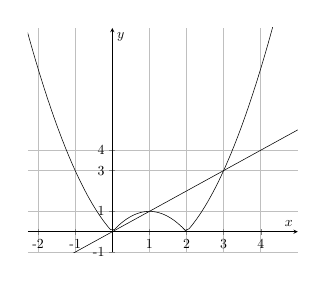
\begin{tikzpicture}[scale=0.5]
\begin{axis}[
    axis lines = middle,
    grid=major,
    legend pos={south west},
    xlabel = {$x$},
    %xlabel style={below right},
    ylabel = {$y$},
    ymin=-1,
    ymax=10,
    xtick={-2,-1,1,2, 3, 4},
    xticklabels={-2,-1,1,2, 3, 4},
    ytick={-2,-1,1, 3, 4},
    yticklabels={-2,-1,1, 3, 4},
                  ]
	\addplot[domain=-5:5, samples=100, color=black] {abs(x*x-2*x)};
    %\addplot[domain=-0.99:0.5, samples=100, color=black] {1/(1-x)};
    \addplot[domain=-5:5, samples=100, color=black] {x};
   % \addplot[domain=1.01:5, samples=100, color=black] {3/(x+1)};
    %\addlegendentry{$\text{Рис. 1}$};
\end{axis}
%\draw (2.75,2.82) circle (2pt);
%\draw (4.11,3.98) circle (2pt);
\end{tikzpicture}$$
 По графику найдём ответ $x \in [1;3]\cup\{0\}.$\\
73. $\cfrac{(x^2-3x+8)(x^2-3x+1)}{x^2-3x}\geqslant3.$ Сделаем замену $t=x^2-3x,$ тогда $\cfrac{(t+8)(t+1)}{t}\geqslant3\Leftrightarrow$\\$
\cfrac{t^2+t+8t+8-3t}{t}\geqslant0\Leftrightarrow \cfrac{t^2+6t+8}{t}\geqslant0\Leftrightarrow \cfrac{(t+2)(t+4)}{t}\geqslant0.$ Применив метод интервалов, найдём ответ: $t\in[-4;-2]\cup(0;+\infty).$
{{PIC:ner9-73.png}}\\
Теперь необходимо решить неравенства относительно $x:\ t\in[-4;-2]\Leftrightarrow\begin{cases} x^2-3x\geqslant-4,\\ x^2-3x\leqslant-2.\end{cases}
\Leftrightarrow\begin{cases} x^2-3x+4\geqslant0,\\ x^2-3x+2\leqslant0.\end{cases}\Leftrightarrow
\begin{cases} (x-1,5)^2+1,75\geqslant0,\\ (x-2)(x-1)\leqslant0.\end{cases}\Rightarrow x\in[1;2].$ Для второго интервала получим $t>0,\ x^2-3x>0,\ x(x-3)>0,\
x\in(-\infty;0)\cup(3;+\infty).$ Таким образом,  $x\in(-\infty;0)\cup[1;2]\cup(3;+\infty).$\\
74. $\cfrac{x\sqrt{x}+x-5\sqrt{x}+2}{\sqrt{x}-2}\geqslant x \Leftrightarrow \begin{cases} t=\sqrt{x}\geqslant0,\\ \cfrac{t^3+t^2-5t+2}{t-2}\geqslant t^2.\end{cases}
\Leftrightarrow \begin{cases} t=\sqrt{x}\geqslant0,\\ \cfrac{t^3+t^2-5t+2}{t-2}\geqslant t^2.\end{cases}
\Leftrightarrow$\\$ \begin{cases} t=\sqrt{x}\geqslant0,\\ \cfrac{t^3+t^2-5t+2-t^3+2t^2}{t-2}\geqslant 0.\end{cases}
\Leftrightarrow \begin{cases} t=\sqrt{x}\geqslant0,\\ \cfrac{3t^2-5t+2}{t-2}\geqslant 0.\end{cases}
\Leftrightarrow \begin{cases} t=\sqrt{x}\geqslant0,\\ \cfrac{(t-1)(3t-2)}{t-2}\geqslant 0.\end{cases}$ Применив метод интервалов, найдём ответ: $t\in\left[\cfrac{2}{3};1\right]\cup(2;+\infty)\Leftrightarrow x \in\left[\cfrac{4}{9};1\right]\cup(4;+\infty).$
{{PIC:int9-74.png}}\\
75. $\cfrac{x\sqrt{x}-x-5\sqrt{x}+3}{\sqrt{x}-3}\geqslant x \Leftrightarrow \begin{cases} t=\sqrt{x}\geqslant0,\\ \cfrac{t^3-t^2-5t+3}{t-3}\geqslant t^2.\end{cases}
\Leftrightarrow \begin{cases} t=\sqrt{x}\geqslant0,\\ \cfrac{t^3+t^2-5t+2}{t-3}\geqslant t^2.\end{cases}
\Leftrightarrow$\\$ \begin{cases} t=\sqrt{x}\geqslant0,\\ \cfrac{t^3-t^2-5t+3-t^3+3t^2}{t-3}\geqslant 0.\end{cases}
\Leftrightarrow \begin{cases} t=\sqrt{x}\geqslant0,\\ \cfrac{2t^2-5t+3}{t-3}\geqslant 0.\end{cases}
\Leftrightarrow \begin{cases} t=\sqrt{x}\geqslant0,\\ \cfrac{(t-1)(2t-3)}{t-3}\geqslant 0.\end{cases}$ Применив метод интервалов, найдём ответ: $t\in\left[1;\cfrac{3}{2}\right]\cup(3;+\infty)\Leftrightarrow x \in\left[1;\cfrac{9}{4}\right]\cup(9;+\infty).$
{{PIC:ner9-75.png}}\\
76. Если знаменатель правой части отрицателен $(x<2),$ то левая часть больше при любом $x$ из области определения: $x^2-5x+6=(x-2)(x-3)\neq0,\ x\neq2$ и $x\neq3.$ Значит, подходит интервал $(-\infty;2).$ Если знаменатель правой дроби положителен $(x>2),$ то необходимо выполнение неравенства $|x^2-5x+6|\leqslant x-2\Leftrightarrow \begin{cases} x^2-5x+6\leqslant x-2,\\ x^2-5x+6\geqslant 2-x.\end{cases}\Leftrightarrow \begin{cases} x^2-6x+8\leqslant0,\\ x^2-4x+4\geqslant0.\end{cases}
\Leftrightarrow \begin{cases} (x-2)(x-4)\leqslant0,\\ (x-2)^2\geqslant0.\end{cases}\Rightarrow x\in(2;3)\cup(3;4].$ Таким образом, итоговый ответ $x\in(-\infty;2)\cup (2;3)\cup(3;4].$\newpage\noindent
77. $\cfrac{(x^2-7x+10)(x^2-8x+16)}{\sqrt{x+10}(-2x^2+3x-10)}\leqslant 0\Leftrightarrow \cfrac{(x-5)(x-2)(x-4)^2}{\sqrt{x+10}(x^2+(x-1,5)^2+7,75)}\geqslant 0.$
Применив метод интервалов, найдём ответ: $x\in(-10;2]\cup\{4\}\cup[5;+\infty).$
{{PIC:ner9-77.png}}\\
78. $(x-1)x(x+1)(x+2)\leqslant8\Leftrightarrow (x^2+x-2)(x^2+x)\leqslant8.$ Сделаем замену $t=x^2+x,$ тогда $(t-2)t\leqslant8\Leftrightarrow
t^2-2t-8\leqslant0\Leftrightarrow(t-4)(t+2)\leqslant0\Leftrightarrow t\in[-2;4]\Leftrightarrow \begin{cases} x^2+x\geqslant-2,\\ x^2+x\leqslant 4.\end{cases}
\Leftrightarrow \begin{cases} x^2+x+2\geqslant0,\\ x^2+x-4\leqslant 0.\end{cases}\Leftrightarrow \left(x-\cfrac{-1-\sqrt{17}}{2}\right)\left(x-\cfrac{-1+\sqrt{17}}{2}\right)\leqslant0\Leftrightarrow x\in \left[\cfrac{-1-\sqrt{17}}{2};\cfrac{-1+\sqrt{17}}{2}\right].$ Целыми решениями этого неравенства являются числа от $-2$ до 1, их сумма равна $-2.$\\
79. Пусть $t=\left|\cfrac{2x-1}{x+2}\right|\geqslant0.$ Тогда $t^2+t\geqslant12,\ (t-3)(t+4)\geqslant0,\ t\geqslant3.$ Значит, $\left|\cfrac{2x-1}{x+2}\right|\geqslant3\Leftrightarrow\left[\begin{array}{l}\cfrac{2x-1}{x+2}\geqslant3,\\ \cfrac{2x-1}{x+2}\leqslant-3.\end{array}\right.
\Leftrightarrow\left[\begin{array}{l}\cfrac{-x-7}{x+2}\geqslant0,\\ \cfrac{5x+5}{x+2}\leqslant0.\end{array}\right.
\Leftrightarrow\left[\begin{array}{l}\cfrac{x+7}{x+2}\leqslant0,\\ \cfrac{x+1}{x+2}\leqslant0.\end{array}\right.
\Leftrightarrow\left[\begin{array}{l}x\in[-7;-2),\\ x\in(-2;-1].\end{array}\right.\Leftrightarrow
x\in[-7;-2)\cup(-2;-1].$\\
80. Пусть $t=\left|\cfrac{2x+3}{x-2}\right|\geqslant0.$ Тогда $t^2\leqslant20+t,\ (t-5)(t+4)\leqslant0,\ t\leqslant5.$ Значит, $\left|\cfrac{2x+3}{x-2}\right|\leqslant5\Leftrightarrow\begin{cases}\cfrac{2x+3}{x-2}\leqslant5,\\ \cfrac{2x+3}{x-2}\geqslant-5.\end{cases}
\Leftrightarrow\begin{cases}\cfrac{-3x+13}{x-2}\leqslant0,\\ \cfrac{7x-7}{x-2}\geqslant0.\end{cases}
\Leftrightarrow\begin{cases}\cfrac{3x-13}{x-2}\geqslant0,\\ \cfrac{x-1}{x-2}\geqslant0.\end{cases}
\Leftrightarrow\begin{cases}x\in[-\infty;2)\cup\left[\cfrac{13}{3};+\infty\right),\\ x\in(-\infty;1]\cup(2;+\infty).\end{cases}\Leftrightarrow
x\in(-\infty;1]\cup\left[\cfrac{13}{3};+\infty\right).$\\
81. $\cfrac{(6-x-x^2)\sqrt{x-1}}{x-3}\geqslant0\Leftrightarrow\cfrac{(2-x)(x+3)\sqrt{x-1}}{x-3}\geqslant0.$ Применив метод интервалов, найдём ответ: $x\in\{1\}\cup[2;3).$
{{PIC:ner9-82.png}}\newpage\noindent
82. $\cfrac{(x^2+3x-18)\sqrt{5-x}}{1-x}\geqslant0\Leftrightarrow\cfrac{(x+6)(x-3)\sqrt{5-x}}{1-x}\geqslant0.$ Применив метод интервалов, найдём ответ: $x\in(-\infty;-6]\cup(1;3)\cup\{5\}.$
{{PIC:ner9-83.png}}\\
83. $(x^2-4x-5)\left(\cfrac{x}{x^2-5x+6}+\cfrac{5}{x^2-10x+21}+\cfrac{7}{(x-2)(x-3)(x-7)}\right)\geqslant0\Leftrightarrow$\\$
(x-5)(x+1)\left(\cfrac{x}{(x-2)(x-3)}+\cfrac{5}{(x-3)(x-7)}+\cfrac{7}{(x-2)(x-3)(x-7)}\right)\geqslant0\Leftrightarrow$\\$
(x-5)(x+1)\cdot\cfrac{x^2-7x+5x-10+7}{(x-2)(x-3)(x-7)}\geqslant0\Leftrightarrow
\cfrac{(x-5)(x+1)(x^2-2x-3)}{(x-2)(x-3)(x-7)}\geqslant0\Leftrightarrow
\cfrac{(x-5)(x+1)^2(x-3)}{(x-2)(x-3)(x-7)}\geqslant0.$ Применив метод интервалов, найдём ответ: $x\in\{-1\}\cup(2;3)\cup(3;5]\cup(7;+\infty).$
{{PIC:ner9-833.png}}\\
84. $\cfrac{|x+2|}{x^2-1}\leqslant-2\Rightarrow x^2-1<0\Rightarrow \begin{cases}x+2>0,\\ (x+1)(x-1)<0.\end{cases} \Rightarrow\begin{cases}|x+2|=x+2,\\ x\in (-1;1).\end{cases}.$ Тогда должно выполняться неравенство $x+2\geqslant 2-2x^2 \Leftrightarrow 2x^2+x \geqslant 0 \Leftrightarrow
x(2x+1)\geqslant 0 \Leftrightarrow x\in\left(\-\infty;-\cfrac{1}{2}\right]\cup[0;+\infty).$ С учётом ранее полученного ограничения имеем ответ $x\in \left(-1;-\cfrac{1}{2}\right]\cup[0;1).$\\
85. $\cfrac{|x+8|}{x^2-4}\leqslant-2\Rightarrow x^2-4<0\Rightarrow \begin{cases}x+8>0,\\ (x+2)(x-2)<0.\end{cases} \Rightarrow\begin{cases}|x+8|=x+8,\\ x\in (-2;2).\end{cases}.$ Тогда должно выполняться неравенство $x+8\geqslant 8-2x^2 \Leftrightarrow 2x^2+x \geqslant 0 \Leftrightarrow
x(2x+1)\geqslant 0 \Leftrightarrow x\in\left(\-\infty;-\cfrac{1}{2}\right]\cup[0;+\infty).$ С учётом ранее полученного ограничения имеем ответ $x\in \left(-2;-\cfrac{1}{2}\right]\cup[0;2).$\newpage\noindent
86. $\cfrac{(x-2)(x-3)^2}{x-1}\geqslant x^2-3x\Leftrightarrow \cfrac{(x-2)(x-3)^2-(x-3)x(x-1)}{x-1}\geqslant0\Leftrightarrow$\\
$\cfrac{(x-3)((x-2)(x-3)-x(x-1))}{x-1}\geqslant0\Leftrightarrow\cfrac{(x-3)(x^2-5x+6-x^2+x)}{x-1}\geqslant0
\Leftrightarrow \cfrac{2(x-3)(3-2x)}{x-1}\geqslant0.$ Применив метод интервалов, найдём ответ: $x\in(-\infty;1)\cup\left[\cfrac{3}{2};3\right].$
{{PIC:ner9-84.png}}\\
87. $\cfrac{(x+1)(x-2)^2}{x+2}\leqslant x^2-2x\Leftrightarrow \cfrac{(x+1)(x-2)^2-(x-2)x(x+2)}{x+2}\leqslant0\Leftrightarrow$\\
$\cfrac{(x-2)((x+1)(x-2)-x(x+2))}{x+2}\leqslant0\Leftrightarrow\cfrac{(x-2)(x^2-x-2-x^2-2x)}{x+2}\leqslant0
\Leftrightarrow \cfrac{(x-2)(3x+2)}{x+2}\geqslant0.$ Применив метод интервалов, найдём ответ: $x\in\left(-2;-\cfrac{2}{3}\right]\cup[2;+\infty).$
{{PIC:ner9-85.png}}\\
88. $2x^2+4xy+4y^2+1\leqslant 2x\Leftrightarrow x^2-2x+1+x^2+4xy+4y^2\leqslant0
\Leftrightarrow (x-1)^2+(x+2y)^2\leqslant0 \Leftrightarrow \begin{cases} x=1,\\ x+2y=0.\end{cases} \Leftrightarrow \begin{cases} x=1,\\ y=-\cfrac{1}{2}.\end{cases}$\\
89.  $\cfrac{2|x|}{x+1}>-x.$ Если $x>0,$ то левая часть неравенства положительна, а правая отрицательна, поэтому все $x>0$ подходят и надо разобрать только случай $x<0$ (тогда $|x|=-x$). Значение $x=0$ не подходит, так как в этом случае левая часть равна правой.

$\cfrac{-2x}{x+1}>-x\Leftrightarrow \cfrac{-2x+x^2+x}{x+1}>0\Leftrightarrow \cfrac{x(x-1)}{x+1}>0.$ Так как $x<0,$ то и $x-1<0,$ а значит необходимо, чтобы выполнялось неравенство $x+1>0,$ то есть $x>-1.$ Таким образом, окончательным ответом является $x\in(-1;0)\cup (0;+\infty).$\\
90. $\cfrac{(2x^2+4x)(3x-x^2)}{(2x+5)^3}\leqslant 0\Leftrightarrow
\cfrac{2x(x+2)x(3-x)}{(2x+5)^3}\leqslant0\Leftrightarrow
\cfrac{x^2(x+2)(x-3)}{(2x+5)^3}\geqslant0.$ Применив метод интервалов, найдём ответ: $x\in\left(-\cfrac{5}{2};-2\right]\cup\{0\}\cup[3;+\infty).$
{{PIC:ner9-86.png}}\\
91. $\cfrac{(x-x^2)(3x^2+15x)}{(2x-7)^3}\geqslant 0\Leftrightarrow
\cfrac{x(1-x)3x(x+5)}{(2x-7)^3}\geqslant0\Leftrightarrow
\cfrac{x^2(x+5)(x-1)}{(2x-7)^3}\leqslant0.$ Применив метод интервалов, найдём ответ: $x\in\left(-\infty;-5\right]\cup\{0\}\cup\left[1;\cfrac{7}{2}\right).$
{{PIC:ner9-87.png}}\\
92. $\left|\cfrac{x-3}{x+4}\right|<1\Leftrightarrow
\begin{cases} \cfrac{x-3}{x+4}<1,\\
\cfrac{x-3}{x+4}>-1.\end{cases}\Leftrightarrow
\begin{cases} \cfrac{x-3-x-4}{x+4}<0,\\
\cfrac{x-3+x+4}{x+4}>0.\end{cases}\Leftrightarrow
\begin{cases} \cfrac{-7}{x+4}<0,\\
\cfrac{2x+1}{x+4}>0.\end{cases}\Leftrightarrow$\\$
\begin{cases} x>-4,\\
x\in(-\infty;-4)\cup\left(-\cfrac{1}{2};+\infty\right).\end{cases}\Leftrightarrow
x\in\left(-\cfrac{1}{2};+\infty\right).$\\
93. $\left|\cfrac{2x+1}{x-1}\right|>2\Leftrightarrow
\left[\begin{array}{l} \cfrac{2x+1}{x-1}>2,\\ \cfrac{2x+1}{x-1}<-2.\end{array}\right.\Leftrightarrow
\left[\begin{array}{l} \cfrac{2x+1-2x+2}{x-1}>0,\\ \cfrac{2x+1+2x-2}{x-1}<0.\end{array}\right.\Leftrightarrow
\left[\begin{array}{l} \cfrac{3}{x-1}>0,\\ \cfrac{4x-1}{x-1}<0.\end{array}\right.\Leftrightarrow$\\$
\left[\begin{array}{l} x>1,\\ x\in\left(\cfrac{1}{4}; 1\right).\end{array}\right.\Leftrightarrow x\in\left(\cfrac{1}{4}; 1\right)\cup(1;+\infty).$\\
94. $\cfrac{3x^2+6x+2}{x^2+2x}+\cfrac{2x+2}{x-1}\geqslant\cfrac{5x+1}{x}
\Leftrightarrow 3+\cfrac{2}{x^2+2x}+2+\cfrac{4}{x-1}\geqslant 5+\cfrac{1}{x}
\Leftrightarrow \cfrac{2}{x(x+2)}+\cfrac{4}{x-1}-\cfrac{1}{x}\geqslant0
\Leftrightarrow \cfrac{2(x-1)+4x(x+2)-(x-1)(x+2)}{x(x+2)(x-1)}\geqslant0
\Leftrightarrow \cfrac{2x-2+4x^2+8x-x^2-2x+x+2}{x(x+2)(x-1)}\geqslant0
\Leftrightarrow \cfrac{3x^2+9x}{x(x+2)(x-1)}\geqslant0
\Leftrightarrow \cfrac{3x(x+3)}{x(x+2)(x-1)}\geqslant0.$ Применив метод интервалов, найдём ответ: $x\in[-3;-2)\cup(1;+\infty).$
{{PIC:ner9-38.png}}\\
95. $\cfrac{(-1+x^2)(x+1)^2(x-1)^3}{x^8-x^6+x^4}\leqslant0\Leftrightarrow\cfrac{(x-1)^4(x+1)^3}{x^4(x^4-x^2+1)}\leqslant0.$ Применив метод интервалов, найдём ответ: $x\in(-\infty;-1]\cup\{1\}.$
{{PIC:ner99-33.png}}
\newpage
